\documentclass[conference]{IEEEtran}
\IEEEoverridecommandlockouts

\usepackage{cite}
\usepackage{amsmath,amssymb}
\usepackage{graphicx}
\usepackage{booktabs}
\usepackage{multirow}
\usepackage{url}
\usepackage[hidelinks]{hyperref}

\graphicspath{{figures/}}

\begin{document}

\title{Physically Realizable Adversarial Patch Attacks on UAS Object Detection:\\
Effectiveness, Transferability, and Robustness}

\author{\IEEEauthorblockN{Mohnish M (AE22B021)}
\IEEEauthorblockA{\textit{AE5510: Security of Safety-Critical Systems}\\
Department of Aerospace Engineering\\
Indian Institute of Technology Madras, Chennai, India}}

\maketitle

\begin{abstract}
Uncrewed aircraft systems (UAS) increasingly rely on deep-learning object detectors for
target recognition, which exposes them to adversarial manipulation in the physical world.
We study an \emph{object-disappearance} attack: a single universal patch, placed on top of
a target, that suppresses its detection by an aerial detector. We fine-tune YOLOv8s on a
four-class aerial dataset (Aircraft, Building, Military Truck, Tank) and optimize a
$300\times300$ patch with Expectation over Transformation (random rotation, scale,
position, brightness, contrast and noise) and a total-variation smoothness penalty. With the
patch covering about 9\% of each object, validation mAP@0.5 falls from 0.622 to 0.129
($-79\%$), compared with 0.376 ($-40\%$) for a random-noise patch of the same size and
placement, showing the effect comes from the learned pattern rather than occlusion. The
patch, which converges to a vegetation-like camouflage texture, transfers without
modification to unseen detectors (YOLOv8n and YOLO11s); a patch trained against a two-model
ensemble matches the single-model patch on its source detector and gives a modest further
transfer gain on validation. In simulation the patch remains effective
under patch rotation, scene brightness from $\times0.5$ to $\times1.5$, a $4\times$
resolution reduction, heavy JPEG compression, and perspective distortion. Its main
limitations are reduced efficacy in dark scenes and on oblique views of vehicles whose
sides remain visible.
\end{abstract}

\begin{IEEEkeywords}
adversarial patch, object detection, UAS, YOLO, expectation over transformation,
physical attacks, transferability
\end{IEEEkeywords}

% ===========================================================================
\section{Introduction}
Deep neural networks are vulnerable to small, deliberately crafted input perturbations
\cite{szegedy2014intriguing,goodfellow2015explaining}. For systems that act in the physical
world, the most relevant threat is not a pixel-level perturbation of a stored image but a
\emph{physically realizable} one: an object that, once placed in the scene, changes what the
camera-based model perceives. Brown \emph{et al.} showed that a small printed patch can
hijack an image classifier regardless of scene \cite{brown2017adversarial}, and later work
extended such patches to object detectors \cite{lee2019physical,thys2019fooling}, including
aerial detection of military assets \cite{denhollander2020adversarial}.

UAS are a natural target: onboard detectors identify aircraft, vehicles, and structures, and
an adversary on the ground controls what those detectors see. An attack that makes a vehicle
or building ``disappear'' from an autonomous UAS's perception is the machine-learning analogue
of camouflage netting, but engineered against a learned model instead of human vision.

This report presents a complete study of such an attack on a UAS detection pipeline:
\begin{itemize}
\item a fine-tuned YOLOv8s baseline on a four-class aerial dataset, with a data audit that
corrected the class mapping and recovered 3\% of training images;
\item a universal object-disappearance patch trained with Expectation over Transformation
(EOT) \cite{athalye2018synthesizing} and total-variation (TV) regularization;
\item an evaluation against a \emph{random-noise control} of identical size and placement,
separating adversarial effect from plain occlusion;
\item a patch-size sweep, a transferability study on two unseen detectors, an ensemble-trained
patch, and a one-factor-at-a-time robustness study (rotation, lighting, resolution,
compression, perspective).
\end{itemize}

% ===========================================================================
\section{Related Work}
\textbf{Adversarial patches.} Brown \emph{et al.} \cite{brown2017adversarial} introduced
universal, scene-independent patches for classification. Athalye \emph{et al.}
\cite{athalye2018synthesizing} proposed EOT, optimizing over a distribution of
transformations so that perturbations survive real-world variation; Sharif \emph{et al.}
\cite{sharif2016accessorize} added printability and smoothness constraints.

\textbf{Attacks on detectors.} Lee and Kolter \cite{lee2019physical} showed that a single
patch can suppress almost all YOLOv3 detections in a scene. Thys \emph{et al.}
\cite{thys2019fooling} optimized a patch that hides people from YOLOv2 by minimizing the
detector's objectness and class scores, with TV and non-printability penalties.

\textbf{Aerial and military targets.} den Hollander \emph{et al.}
\cite{denhollander2020adversarial} camouflaged military assets in overhead imagery against
YOLOv2 and observed that patches trained over full rotation tend toward rotationally symmetric
patterns, consistent with our findings (Section~\ref{sec:attackres}).

\textbf{Optical attacks.} Gnanasambandam \emph{et al.} \cite{gnanasambandam2021optical}
projected adversarial light patterns onto objects instead of printing them, an alternative
physical channel relevant to future work.

\textbf{Transferability.} Adversarial examples often transfer between models, and optimizing
against an ensemble of models improves black-box transfer \cite{liu2017delving}.

% ===========================================================================
\section{Dataset and Data Audit}
\label{sec:data}
The dataset contains aerial images of four object classes, provided with YOLO-format labels
(class, normalized box centre, width and height). The training set was pre-augmented
(rotation, scaling, brightness/contrast, flips); it consists of 88 source images, each
augmented 36 times. Table~\ref{tab:data} summarizes the splits.

\begin{table}[t]
\centering
\caption{Dataset splits (after preparation).}
\label{tab:data}
\begin{tabular}{lrrrrrr}
\toprule
Split & Images & Boxes & Airc. & Bldg. & Truck & Tank \\
\midrule
Train & 3168 & 49099 & 16699 & 17983 & 6548 & 7869 \\
Val   & 16   & 106   & 8     & 68    & 23   & 7 \\
Test  & 16   & 132   & 35    & 56    & 22   & 19 \\
\bottomrule
\end{tabular}
\end{table}

Before training we audited the labels and found three issues:
\begin{enumerate}
\item \textbf{Class mapping.} Visual inspection of annotated boxes showed the IDs are
0\,=\,Aircraft, 1\,=\,Building, 2\,=\,Military Truck, 3\,=\,Tank, which differs from the
order in which the dataset documentation lists the classes. Using the documented order would
have mislabelled three of the four classes.
\item \textbf{Out-of-frame boxes.} Rotation augmentation left box coordinates outside
$[0,1]$ in 105 training images. The training framework tolerates only small overshoots
($-0.01$ to $1.01$) and silently discarded 94 of these images, so we clipped boxes to the frame (dropping 149 boxes that lay entirely outside), recovering
all 3168 images.
\item \textbf{Polygon labels.} Four validation annotations were stored as four-corner
polygons; they were converted to their bounding boxes.
\end{enumerate}
The validation and test sets are small (16 images each), so metrics on them have high
variance; in particular, 20 of the 22 test trucks come from a single image
(Section~\ref{sec:baseline}). For the robustness study we therefore pool validation and test
(32 images, 238 objects).

% ===========================================================================
\section{Baseline Detector}
\label{sec:baseline}
We fine-tune YOLOv8s \cite{jocher2023yolov8} from COCO-pretrained weights \cite{lin2014coco}
at $640\times640$ input, batch size 16, with the framework's default augmentation and AdamW
optimizer (learning rate $1.25\times10^{-3}$, selected automatically) and early stopping with
patience 25 on validation mAP@0.5. Training stopped at epoch 50; the best checkpoint
(epoch 25) is used throughout. For the transferability study we train YOLOv8n
\cite{jocher2023yolov8} and YOLO11s \cite{jocher2024yolo11} with the same recipe (best
epochs 8 and 13 respectively). All experiments use one RTX 4060 Laptop GPU (8\,GB).

\begin{table}[t]
\centering
\caption{Baseline detection performance (AP@0.5).}
\label{tab:baseline}
\begin{tabular}{llcc}
\toprule
Model & Metric & Val & Test \\
\midrule
\multirow{8}{*}{YOLOv8s} & Aircraft & 0.819 & 0.694 \\
 & Building & 0.616 & 0.668 \\
 & Military Truck & 0.470 & 0.017 \\
 & Tank & 0.584 & 0.581 \\
\cmidrule{2-4}
 & mAP@0.5 & \textbf{0.622} & \textbf{0.490} \\
 & mAP@0.5:0.95 & 0.409 & 0.261 \\
 & Precision & 0.647 & 0.573 \\
 & Recall & 0.646 & 0.468 \\
\midrule
YOLOv8n & mAP@0.5 & 0.689 & 0.465 \\
YOLO11s & mAP@0.5 & 0.743 & 0.469 \\
\bottomrule
\end{tabular}
\end{table}

Table~\ref{tab:baseline} reports the results. Aircraft is the easiest class. The near-zero
test AP for Military Truck is caused by one oblique photograph of a crowded vehicle display
yard that contains 20 of the 22 test trucks: the detector localizes most of them but labels
them \emph{Building}, as rows of parked vehicles resemble rows of rooftops. On the remaining
truck images detection is correct. Validation mAP fluctuated between 0.32 and 0.64 across
epochs, another consequence of the 16-image validation set.

% ===========================================================================
\section{Attack Method}
\label{sec:method}
\subsection{Threat Model}
The adversary wants a target object to go undetected by the UAS detector
(object disappearance). The adversary can place one printed patch on each target and has
white-box access to the detector during patch optimization (black-box transfer to other
detectors is evaluated in Section~\ref{sec:transfer}). The patch is \emph{universal}: one
pattern is used for every object of every class.

\subsection{Patch Application}
For an image $x$ with ground-truth boxes $\{b_j\}$, the patch $p\in[0,1]^{3\times300\times300}$
is pasted at the centre of each box with side length $s_j = \alpha\sqrt{w_j h_j}$, where
$\alpha$ is the patch scale ($\alpha=0.3$, i.e.\ about 9\% of the box area, unless stated).
Pasting uses a differentiable affine warp $\mathcal{W}$ (bilinear sampling) with mask $M$:
\begin{equation}
x' = (1 - M)\odot x + M\odot \mathcal{W}(t(p)),
\end{equation}
where $t$ is a random transformation drawn from the EOT distribution $\mathcal{T}$.

\subsection{Expectation over Transformation}
During training each pasted copy receives an independent transformation: rotation
$\theta\sim U(0^\circ,360^\circ)$ (aerial views have no canonical heading), scale jitter
$\pm20\%$, translation within the box of $\pm15\%$ of its width/height, contrast
$\times U(0.8,1.2)$, brightness $+U(-0.1,0.1)$, and uniform pixel noise $\pm0.05$.

\subsection{Loss}
Let $s_a=\max_c \sigma(z_{a,c})$ be the highest class score of prediction $a$, and let
$S_i$ be the scores of all predictions in image $i$ whose box centre lies inside a patched
ground-truth box. Taking the maximum over classes means relabelling an object as a different
class does not reduce the loss---the object must vanish. The detection loss is
\begin{equation}
\mathcal{L}_{\text{det}} = \frac{1}{N}\sum_{i=1}^{N}\Big(\max S_i +
\operatorname{mean}\,\operatorname{top}_{k_i}(S_i)\Big),\qquad k_i = 3n_i,
\end{equation}
where $n_i$ is the number of patched objects in image $i$. The maximum term follows
\cite{thys2019fooling}; the top-$k$ term pushes down every object rather than only the most
confident one. A total-variation term \cite{rudin1992nonlinear,sharif2016accessorize}
keeps the patch smooth and printable:
\begin{equation}
\mathcal{L}_{\text{TV}} = \operatorname{mean}|p_{u+1,v}-p_{u,v}| + \operatorname{mean}|p_{u,v+1}-p_{u,v}|,
\end{equation}
and the patch solves
\begin{equation}
p^{*} = \arg\min_{p}\; \mathbb{E}_{t\sim\mathcal{T}}\big[\mathcal{L}_{\text{det}}\big]
+ \lambda_{\text{TV}}\,\mathcal{L}_{\text{TV}},\qquad \lambda_{\text{TV}}=2.5 .
\end{equation}

\subsection{Optimization}
The detector's weights are frozen. The patch is initialized to grey with small Gaussian noise
and optimized with Adam \cite{kingma2015adam} (learning rate 0.02, halved when the epoch loss
plateaus), batch size 8, for 30 epochs ($\approx$11{,}900 steps, $\approx$1.1\,h). At most 24
objects per training image are patched; objects smaller than 12\,px at $640$\,px input are
skipped. Only the training split is used.

\subsection{Evaluation Protocol}
On validation and test images, the converged patch is pasted at the centre of every object
at scale $\alpha$, with a random but fixed rotation per object and no photometric change.
We compare three conditions with identical metrics: \emph{clean} (no patch),
\emph{random noise} (a uniform-noise patch with the same size and placement), and
\emph{adversarial}. The random-noise control is essential: covering part of an object
reduces detection on its own, so only the gap between adversarial and random noise measures
the adversarial effect.

% ===========================================================================
\section{Results}
\subsection{Attack Effectiveness}
\label{sec:attackres}
Table~\ref{tab:attack} and Fig.~\ref{fig:perclass} show the main result. On validation,
mAP@0.5 drops from 0.622 to 0.129 ($-79\%$) under the adversarial patch versus 0.376
($-40\%$) under random noise. On test the drop is 0.490$\to$0.226 ($-54\%$) versus 0.393
($-20\%$). Precision collapses (0.647$\to$0.139 on validation), indicating that the
remaining detections are low-confidence or mislocalized.

\begin{table}[t]
\centering
\caption{AP@0.5 with the patch covering $\approx$9\% of each object (YOLOv8s).
C\,=\,clean, N\,=\,random noise, A\,=\,adversarial.}
\label{tab:attack}
\setlength{\tabcolsep}{4pt}
\begin{tabular}{lcccccc}
\toprule
 & \multicolumn{3}{c}{Validation} & \multicolumn{3}{c}{Test} \\
\cmidrule(lr){2-4}\cmidrule(lr){5-7}
Class & C & N & A & C & N & A \\
\midrule
Aircraft & 0.819 & 0.188 & \textbf{0.090} & 0.694 & 0.726 & \textbf{0.182} \\
Building & 0.616 & 0.290 & \textbf{0.114} & 0.668 & 0.221 & \textbf{0.074} \\
Mil.\ Truck & 0.470 & 0.339 & \textbf{0.194} & 0.017 & 0.001 & 0.000 \\
Tank & 0.584 & 0.688 & \textbf{0.119} & 0.581 & 0.625 & 0.648 \\
\midrule
mAP@0.5 & 0.622 & 0.376 & \textbf{0.129} & 0.490 & 0.393 & \textbf{0.226} \\
Recall & 0.646 & 0.478 & 0.312 & 0.468 & 0.396 & 0.263 \\
\bottomrule
\end{tabular}
\end{table}

\begin{figure*}[t]
\centering
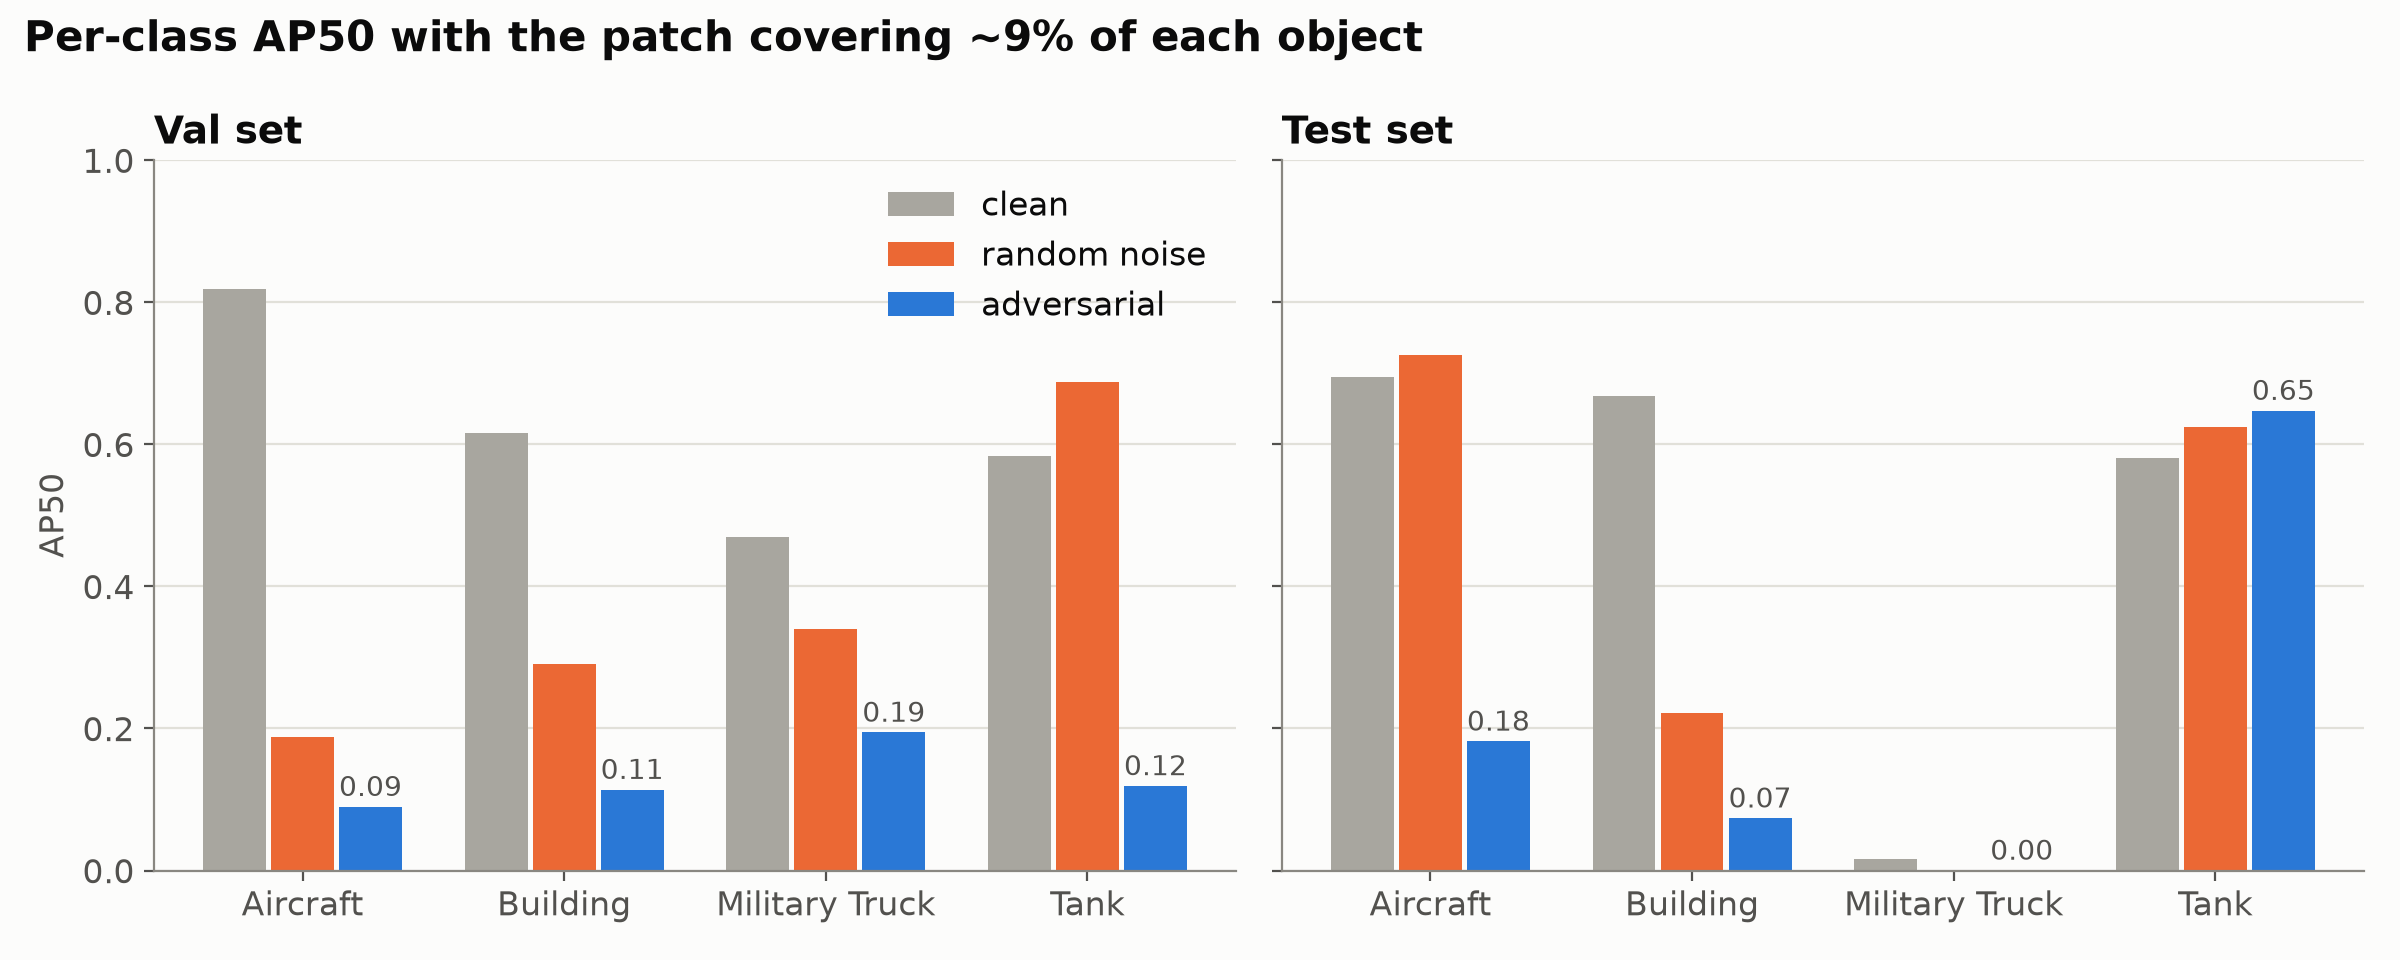
\includegraphics[width=0.9\textwidth]{per_class.png}
\caption{Per-class AP@0.5 for clean images, a random-noise patch, and the adversarial patch
(patch covers $\approx$9\% of each object). Numbers above the blue bars give adversarial AP.}
\label{fig:perclass}
\end{figure*}

Aircraft and Building are suppressed on both splits. Tanks are suppressed on validation
(0.584$\to$0.119) but not on test, where they are unaffected (0.581$\to$0.648). All test
tanks received a patch; the test tank photographs are low, oblique views in which the hull
side, tracks and gun barrel remain visible around a flat, roof-mounted patch, whereas
training images are predominantly overhead. Test trucks cannot be assessed because their
clean AP is already near zero (Section~\ref{sec:baseline}).

Fig.~\ref{fig:evolution} shows the patch during optimization. Starting from noise, it
converges to a smooth green, vegetation-like texture with roughly circular structures. The
detector appears to associate this texture with ground cover, so the patch makes objects
blend into the background---an emergent form of camouflage. The circular structure is
consistent with den Hollander \emph{et al.}'s observation for rotation-trained patches
\cite{denhollander2020adversarial}. Fig.~\ref{fig:beforeafter} shows detections before and
after patching. On an airport apron, all eight aircraft are detected in the clean image
(confidence 0.71--0.84); with the patch only three of the eight are found, all weakly
($\leq$0.55). Buildings fail differently: the detector still fires, producing more boxes than
on the clean image (35 vs.\ 25), but they no longer align with real buildings, and correctly
localized detections (IoU\,$\geq$\,0.5) fall from 10 to 1 of 17. The patch thus suppresses
some objects and scrambles the localization of others, consistent with the collapse in
precision.

\begin{figure*}[t]
\centering
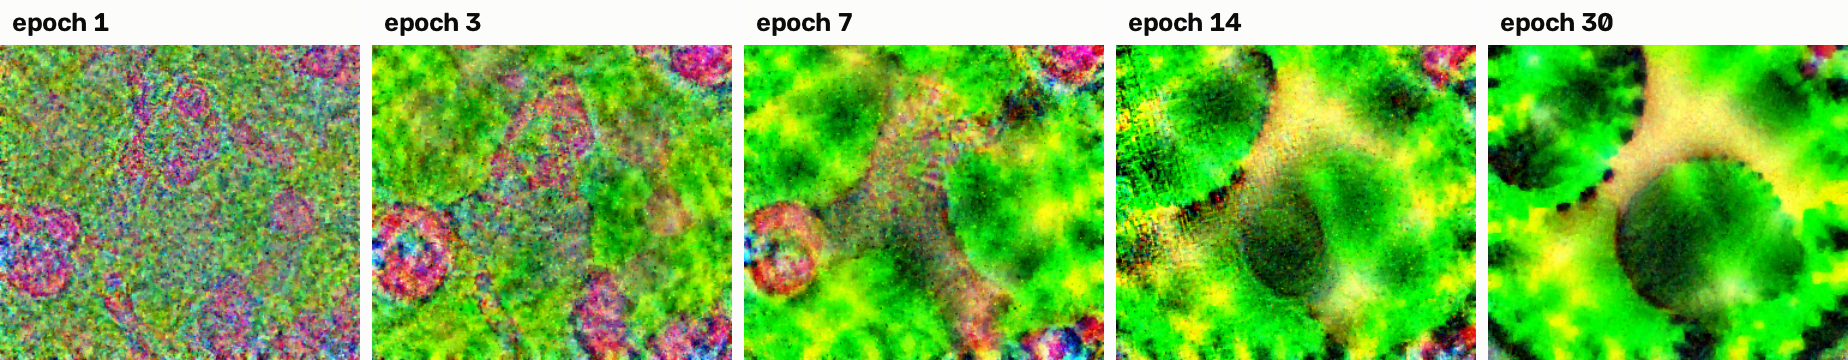
\includegraphics[width=0.95\textwidth]{patch_evolution.png}
\caption{Patch at selected training epochs. Noise turns into a vegetation-like camouflage
texture; the loss plateaus after roughly epoch 14.}
\label{fig:evolution}
\end{figure*}

\begin{figure}[t]
\centering
\includegraphics[width=\columnwidth]{before_after.png}
\caption{YOLOv8s detections on test images without (left) and with (right) the adversarial
patch. Top: 3 of 8 aircraft remain detected, all weakly. Bottom: boxes no longer align with
buildings; correct detections fall from 10 to 1 of 17.}
\label{fig:beforeafter}
\end{figure}

\subsection{Effect of Patch Size}
Without retraining, we evaluate the same patch at four sizes (Fig.~\ref{fig:size},
Table~\ref{tab:size}). The adversarial patch is far more damaging than random noise at every
size: at only 4\% coverage it halves validation mAP (0.622$\to$0.299, versus 0.506 for
noise), and at 16\% coverage it reduces validation mAP to 0.053.

\begin{table}[t]
\centering
\caption{mAP@0.5 versus patch size (YOLOv8s). N\,=\,random noise, A\,=\,adversarial.}
\label{tab:size}
\begin{tabular}{cccccc}
\toprule
 & & \multicolumn{2}{c}{Validation} & \multicolumn{2}{c}{Test} \\
\cmidrule(lr){3-4}\cmidrule(lr){5-6}
$\alpha$ & Coverage & N & A & N & A \\
\midrule
0.1 & 1\%  & 0.618 & 0.535 & 0.484 & 0.447 \\
0.2 & 4\%  & 0.506 & 0.299 & 0.417 & 0.287 \\
0.3 & 9\%  & 0.376 & 0.129 & 0.393 & 0.226 \\
0.4 & 16\% & 0.202 & 0.053 & 0.396 & 0.166 \\
\bottomrule
\multicolumn{6}{l}{\footnotesize Clean: 0.622 (val), 0.490 (test).}
\end{tabular}
\end{table}

\begin{figure*}[t]
\centering
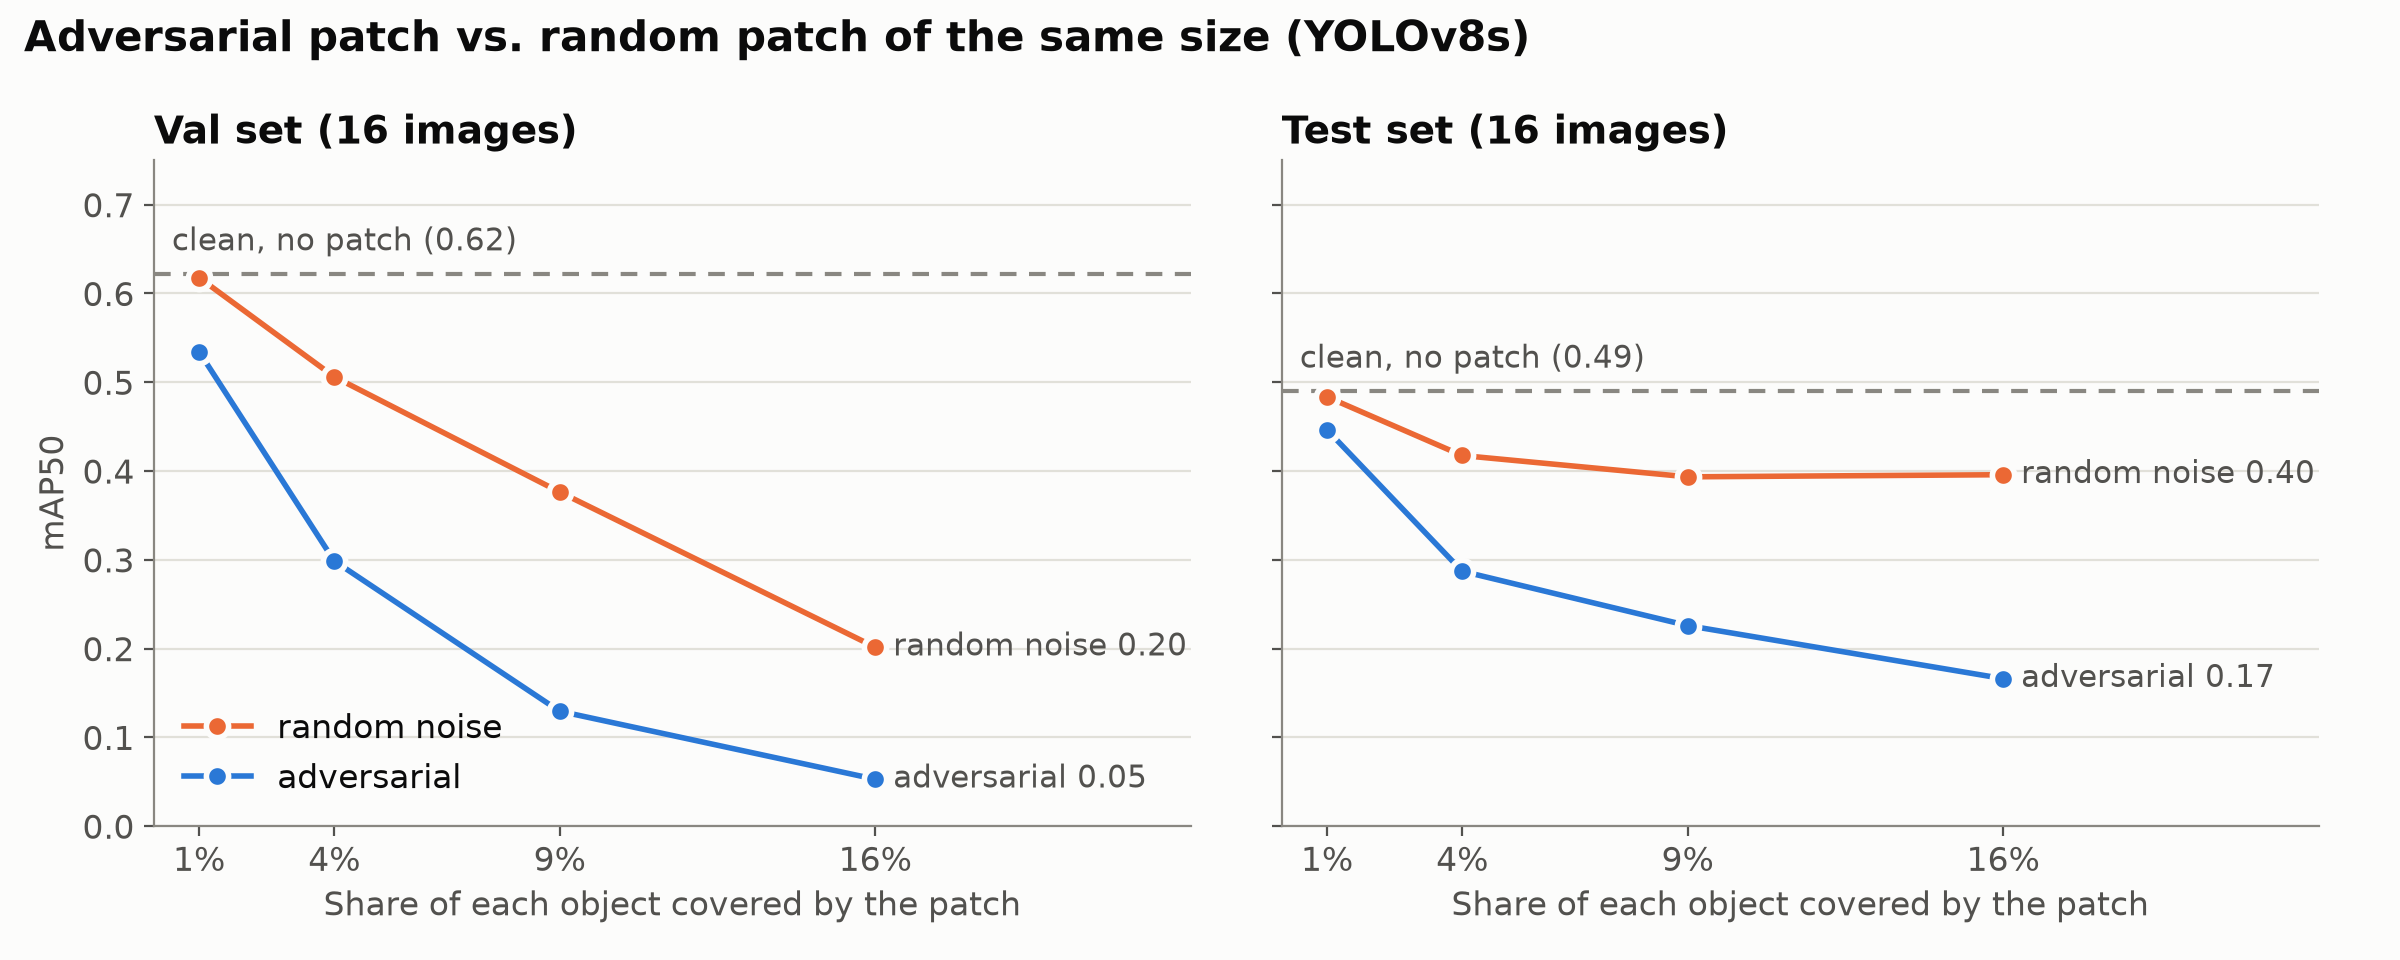
\includegraphics[width=0.9\textwidth]{size_vs_damage.png}
\caption{mAP@0.5 versus share of each object covered by the patch, for the adversarial patch
and a random-noise patch of identical size and placement. Dashed line: clean performance.}
\label{fig:size}
\end{figure*}

\subsection{Transferability}
\label{sec:transfer}
To test whether the attack requires knowledge of the deployed model, the patch optimized on
YOLOv8s is evaluated, unchanged, on YOLOv8n (same family, smaller) and YOLO11s (different
backbone and head), which it never saw (Fig.~\ref{fig:transfer}, Table~\ref{tab:transfer}).

\begin{table}[t]
\centering
\caption{Transfer of the YOLOv8s patch (mAP@0.5, $\alpha=0.3$).}
\label{tab:transfer}
\setlength{\tabcolsep}{4pt}
\begin{tabular}{lcccccc}
\toprule
 & \multicolumn{3}{c}{Validation} & \multicolumn{3}{c}{Test} \\
\cmidrule(lr){2-4}\cmidrule(lr){5-7}
Target & C & N & A & C & N & A \\
\midrule
YOLOv8s (white-box) & 0.622 & 0.376 & 0.129 & 0.490 & 0.393 & 0.226 \\
YOLOv8n (unseen) & 0.689 & 0.517 & 0.409 & 0.465 & 0.400 & 0.308 \\
YOLO11s (unseen) & 0.743 & 0.501 & 0.350 & 0.469 & 0.408 & 0.309 \\
\bottomrule
\end{tabular}
\end{table}

\begin{figure*}[t]
\centering
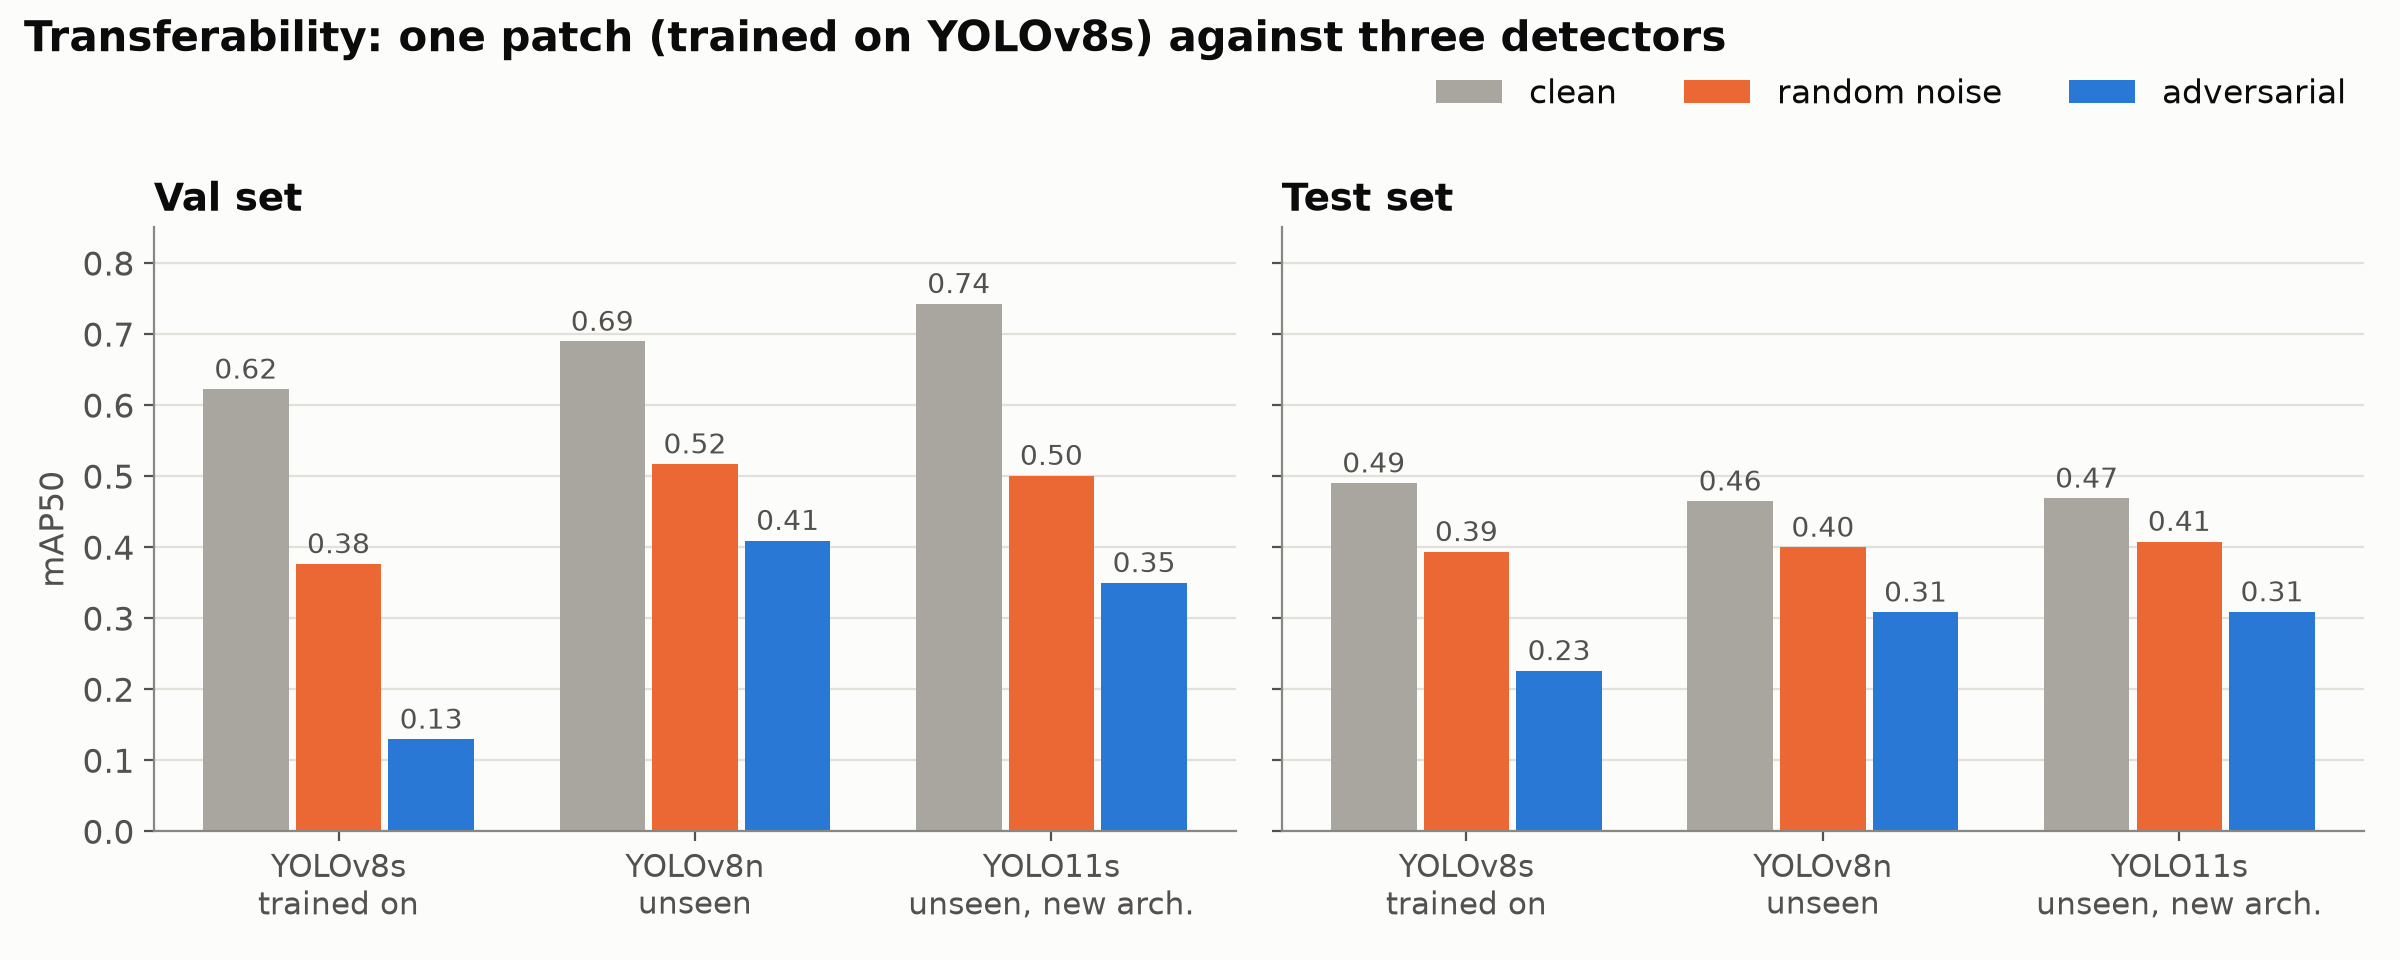
\includegraphics[width=0.9\textwidth]{transfer.png}
\caption{Transferability: the patch optimized on YOLOv8s evaluated on YOLOv8s and two unseen
detectors.}
\label{fig:transfer}
\end{figure*}

The patch transfers partially. On both unseen detectors it reduces mAP well below the
random-noise level (validation: 0.409 vs.\ 0.517 on YOLOv8n; 0.350 vs.\ 0.501 on YOLO11s),
but the additional damage beyond noise is smaller than in the white-box case (0.11--0.15
versus 0.25 on validation). A different architecture did not confer more robustness: YOLO11s
was affected at least as much as YOLOv8n. Transfer is class-dependent. Buildings transfer
strongly (test AP 0.680$\to$0.164 on YOLOv8n and 0.626$\to$0.166 on YOLO11s), aircraft
transfer to YOLO11s (validation 0.955$\to$0.427) but not to YOLOv8n (0.605 adversarial vs.\
0.598 noise), and test tanks resist on every model.

\subsection{Ensemble Patch}
\label{sec:ensemble}
Optimizing against several models is a standard way to improve black-box transfer
\cite{liu2017delving}. We therefore trained a second patch with identical settings against
YOLOv8s and YOLO11s jointly, averaging $\mathcal{L}_{\text{det}}$ over the two detectors
(20 epochs; gradients are accumulated one model at a time, keeping peak GPU memory at
5\,GB). YOLOv8n remains unseen and serves as the transfer target. Table~\ref{tab:ensemble}
compares the two patches.

\begin{table}[t]
\centering
\caption{Single-model vs.\ ensemble patch (mAP@0.5, val\,/\,test, $\alpha=0.3$).
Noise is the random-noise control on the same detector.}
\label{tab:ensemble}
\setlength{\tabcolsep}{3.5pt}
\begin{tabular}{lccc}
\toprule
Target & Noise & Single (v8s) & Ensemble (v8s+11s) \\
\midrule
YOLOv8s (seen by both) & 0.376\,/\,0.393 & 0.129\,/\,0.226 & \textbf{0.122}\,/\,\textbf{0.224} \\
YOLO11s (seen by ens.) & 0.501\,/\,0.408 & 0.350\,/\,0.309 & \textbf{0.246}\,/\,\textbf{0.264} \\
YOLOv8n (unseen) & 0.517\,/\,0.400 & 0.409\,/\,\textbf{0.308} & \textbf{0.354}\,/\,0.317 \\
\bottomrule
\end{tabular}
\end{table}

Sharing one patch between two detectors cost nothing on YOLOv8s (0.122 vs.\ 0.129 on
validation) while substantially strengthening the attack on YOLO11s, as expected once it is
part of the training set. On the unseen YOLOv8n, the ensemble patch improved validation
mAP suppression (0.409$\to$0.354, widening the margin over noise from 0.11 to 0.16) but not
test (0.308 vs.\ 0.317, within the variation expected from 16 images). The ensemble therefore
gives at most a modest transfer gain here; confirming it would require a larger evaluation
set and more held-out detectors.

\subsection{Robustness to Imaging Conditions}
We vary one condition at a time, applying it to the whole image \emph{after} the patch is
pasted, as a camera would observe a physical patch; clean and noise images undergo the same
condition. Validation and test are pooled (32 images, 238 objects). Fig.~\ref{fig:robust}
and Table~\ref{tab:robust} summarize the results using the \emph{retained ratio}
$\text{mAP}_{\text{A}}/\text{mAP}_{\text{C}}$ (lower means a stronger attack).

\begin{table}[t]
\centering
\caption{Robustness (pooled val+test, YOLOv8s). Retained ratio = mAP under the patch divided
by clean mAP under the same condition.}
\label{tab:robust}
\setlength{\tabcolsep}{3.5pt}
\begin{tabular}{llcccc}
\toprule
Factor & Value & Clean & Noise & Adv. & Retained \\
\midrule
Rotation & 0$^\circ$--180$^\circ$ & 0.538 & 0.36--0.42 & 0.18--0.20 & 0.34--0.37 \\
\midrule
\multirow{3}{*}{Brightness} & $\times$0.5 & 0.563 & 0.431 & 0.269 & 0.48 \\
 & $\times$1.0 & 0.538 & 0.394 & 0.207 & 0.38 \\
 & $\times$1.5 & 0.500 & 0.369 & 0.158 & 0.32 \\
\midrule
\multirow{3}{*}{Resolution} & 100\% & 0.538 & 0.394 & 0.207 & 0.38 \\
 & 50\% & 0.539 & 0.451 & 0.234 & 0.44 \\
 & 25\% & 0.454 & 0.282 & 0.183 & 0.40 \\
\midrule
\multirow{3}{*}{JPEG quality} & 95 & 0.541 & 0.380 & 0.213 & 0.39 \\
 & 50 & 0.502 & 0.343 & 0.174 & 0.35 \\
 & 10 & 0.432 & 0.292 & 0.128 & 0.30 \\
\midrule
\multirow{3}{*}{Perspective} & 0.0 & 0.538 & 0.394 & 0.207 & 0.38 \\
 & 0.4 & 0.445 & 0.351 & 0.151 & 0.34 \\
 & 0.6 & 0.285 & 0.223 & 0.102 & 0.36 \\
\bottomrule
\end{tabular}
\end{table}

\begin{figure*}[t]
\centering
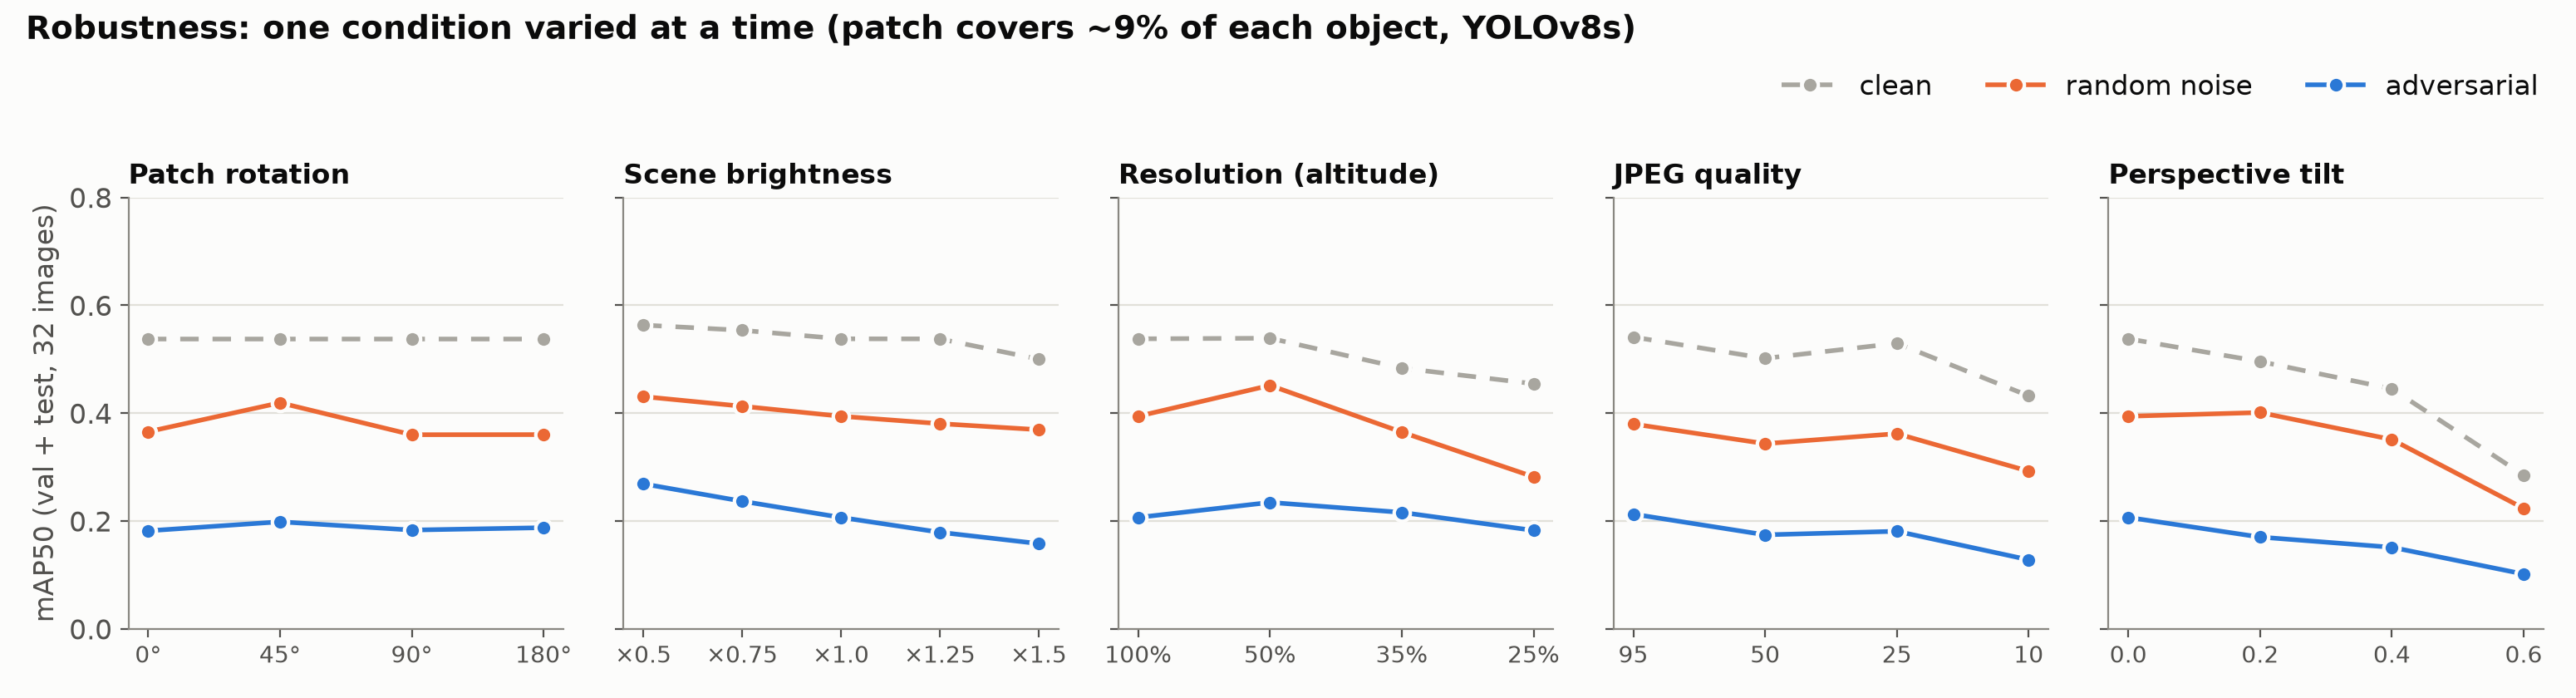
\includegraphics[width=\textwidth]{robustness.png}
\caption{Robustness study: mAP@0.5 on pooled validation and test images as one condition is
varied. Resolution simulates altitude (fewer pixels on target); perspective is a keystone
warp that shrinks the top image edge by the given fraction.}
\label{fig:robust}
\end{figure*}

The attack holds across all tested conditions, with retained ratios of 0.30--0.48 versus
0.62--0.84 for random noise:
\begin{itemize}
\item \textbf{Rotation} has essentially no effect, confirming that rotation EOT produced an
orientation-invariant patch.
\item \textbf{Brightness} is the weakest point: in dark scenes ($\times0.5$) the patch's
colours wash out and the retained ratio rises to 0.48, though still far below noise (0.76).
\item \textbf{Resolution} down to 25\% (simulating a $4\times$ higher altitude) and
\textbf{JPEG compression} down to quality 10 do not neutralize the attack; strong compression
slightly strengthens it.
\item \textbf{Perspective distortion} degrades clean detection substantially, but the
retained ratio stays near 0.35.
\end{itemize}
Test tanks stay detected (AP@0.5 0.33--0.52) under every condition, including perspective
warping, which did not prevent the patch from working on other classes. This supports the
explanation that the tanks' resistance comes from scene content---visible sides and gun
barrels in oblique photographs---rather than from image distortion.

% ===========================================================================
\section{Discussion and Limitations}
\textbf{Security implications.} A single universal, smooth patch covering a few percent of an
object's area suppresses most detections of a fine-tuned UAS detector, survives realistic
variations in viewing and imaging conditions, and transfers to detectors it was not trained
on. Replacing or upgrading the model therefore does not by itself remove the threat; defences
need to address the input (e.g.\ patch or occlusion detection) or the training (e.g.\
adversarial training).

\textbf{Limitations.}
\begin{itemize}
\item \emph{Simulation only.} Lighting, resolution, compression and perspective are applied
in software; no patch was printed and photographed, and printer colour gamut (which a
non-printability score \cite{sharif2016accessorize} would address) was not modelled.
\item \emph{Small evaluation sets.} With 16 images per split (32 pooled), individual images
move metrics substantially; per-class results for Truck and Tank rest on few images.
\item \emph{Flat patch, overhead training data.} The keystone warp only approximates an
oblique view; it cannot reveal a vehicle's sides. The resistance of obliquely photographed
tanks indicates that a single roof-mounted patch is insufficient when the target's
silhouette remains visible.
\item \emph{Annotation quality.} Some rotation-augmented training boxes are loosely aligned
with their objects, which limits baseline accuracy.
\end{itemize}

\textbf{Future work.} Evaluating the ensemble patch on a larger test set and more held-out
detectors, including non-YOLO architectures; widening the brightness range in EOT to address
low-light scenes; multi-face or wrap-around patches for oblique views; light-projection
attacks \cite{gnanasambandam2021optical}; and print-and-photograph validation.

% ===========================================================================
\section{Conclusion}
We fine-tuned a YOLOv8s detector on four-class aerial imagery and showed that a universal,
EOT-trained adversarial patch covering about 9\% of each object reduces validation mAP@0.5
from 0.622 to 0.129, roughly twice the damage of a random patch of the same size. The patch
converges to a vegetation-like camouflage texture, transfers to unseen YOLOv8n and YOLO11s
detectors---more so when trained against an ensemble, although the gain on the unseen model
was small---and remains effective in simulation across rotation, lighting, resolution,
compression and perspective changes. Its main weaknesses---dark scenes and oblique views of
vehicles---point to where physical defences and further attack research should focus.

% ===========================================================================
\begin{thebibliography}{99}

\bibitem{szegedy2014intriguing}
C.~Szegedy, W.~Zaremba, I.~Sutskever, J.~Bruna, D.~Erhan, I.~Goodfellow, and R.~Fergus,
``Intriguing properties of neural networks,'' in \emph{Proc. Int. Conf. Learn.
Representations (ICLR)}, 2014.

\bibitem{goodfellow2015explaining}
I.~J. Goodfellow, J.~Shlens, and C.~Szegedy, ``Explaining and harnessing adversarial
examples,'' in \emph{Proc. Int. Conf. Learn. Representations (ICLR)}, 2015.

\bibitem{brown2017adversarial}
T.~B. Brown, D.~Man\'{e}, A.~Roy, M.~Abadi, and J.~Gilmer, ``Adversarial patch,''
arXiv:1712.09665, 2017.

\bibitem{athalye2018synthesizing}
A.~Athalye, L.~Engstrom, A.~Ilyas, and K.~Kwok, ``Synthesizing robust adversarial examples,''
in \emph{Proc. Int. Conf. Mach. Learn. (ICML)}, 2018, pp. 284--293.

\bibitem{sharif2016accessorize}
M.~Sharif, S.~Bhagavatula, L.~Bauer, and M.~K. Reiter, ``Accessorize to a crime: Real and
stealthy attacks on state-of-the-art face recognition,'' in \emph{Proc. ACM SIGSAC Conf.
Comput. Commun. Secur. (CCS)}, 2016, pp. 1528--1540.

\bibitem{lee2019physical}
M.~Lee and Z.~Kolter, ``On physical adversarial patches for object detection,''
arXiv:1906.11897, 2019.

\bibitem{thys2019fooling}
S.~Thys, W.~Van~Ranst, and T.~Goedem\'{e}, ``Fooling automated surveillance cameras:
Adversarial patches to attack person detection,'' in \emph{Proc. IEEE/CVF Conf. Comput.
Vis. Pattern Recognit. Workshops (CVPRW)}, 2019.

\bibitem{denhollander2020adversarial}
R.~den Hollander \emph{et al.}, ``Adversarial patch camouflage against aerial detection,''
in \emph{Proc. SPIE 11543, Artificial Intelligence and Machine Learning in Defense
Applications II}, 2020.

\bibitem{gnanasambandam2021optical}
A.~Gnanasambandam, A.~M. Sherman, and S.~H. Chan, ``Optical adversarial attack,'' in
\emph{Proc. IEEE/CVF Int. Conf. Comput. Vis. Workshops (ICCVW)}, 2021.

\bibitem{liu2017delving}
Y.~Liu, X.~Chen, C.~Liu, and D.~Song, ``Delving into transferable adversarial examples and
black-box attacks,'' in \emph{Proc. Int. Conf. Learn. Representations (ICLR)}, 2017.

\bibitem{jocher2023yolov8}
G.~Jocher, A.~Chaurasia, and J.~Qiu, ``Ultralytics YOLOv8,'' 2023. [Online]. Available:
\url{https://github.com/ultralytics/ultralytics}

\bibitem{jocher2024yolo11}
G.~Jocher and J.~Qiu, ``Ultralytics YOLO11,'' 2024. [Online]. Available:
\url{https://github.com/ultralytics/ultralytics}

\bibitem{lin2014coco}
T.-Y. Lin, M.~Maire, S.~Belongie, J.~Hays, P.~Perona, D.~Ramanan, P.~Doll\'{a}r, and
C.~L. Zitnick, ``Microsoft COCO: Common objects in context,'' in \emph{Proc. Eur. Conf.
Comput. Vis. (ECCV)}, 2014, pp. 740--755.

\bibitem{rudin1992nonlinear}
L.~I. Rudin, S.~Osher, and E.~Fatemi, ``Nonlinear total variation based noise removal
algorithms,'' \emph{Physica D: Nonlinear Phenomena}, vol.~60, no.~1--4, pp. 259--268, 1992.

\bibitem{kingma2015adam}
D.~P. Kingma and J.~Ba, ``Adam: A method for stochastic optimization,'' in \emph{Proc. Int.
Conf. Learn. Representations (ICLR)}, 2015.

\end{thebibliography}

\end{document}
